% ============================================================
% HSBI Beamer — ISLP Lecture Series — IMPROVED EDITION
% Chapter 7: Moving Beyond Linearity
% ============================================================
\documentclass[aspectratio=169,11pt]{beamer}
\usepackage[utf8]{inputenc}\usepackage[T1]{fontenc}\usepackage[english]{babel}
\usepackage{graphicx}\usepackage{booktabs}\usepackage{amsmath,amssymb,amsfonts}
\usepackage{mathtools}\usepackage{hyperref}\usepackage{xcolor}
\usepackage{verbatim}\usepackage{alltt}
\usepackage{tikz}\usetikzlibrary{calc,arrows.meta,positioning,shapes}
\usepackage{tcolorbox}\tcbuselibrary{skins}

\usetheme{Madrid}\usecolortheme{default}
\setbeamertemplate{navigation symbols}{}
\setbeamertemplate{footline}[frame number]
\setbeamertemplate{blocks}[rounded][shadow=false]
\setbeamertemplate{headline}{%
  \leavevmode\hbox{%
    \begin{beamercolorbox}[wd=\paperwidth,ht=2.2ex,dp=0.9ex]{section in head/foot}%
      {\fontsize{4.6}{5.2}\selectfont%
       \insertsectionnavigationhorizontal{\paperwidth}{}{\hskip0pt plus1filll}}%
    \end{beamercolorbox}}%
}
\setbeamerfont{section in head/foot}{size=\tiny}
\setbeamerfont{palette primary}{size=\tiny}
\setbeamerfont{palette tertiary}{size=\tiny}
\setbeamerfont{section in toc}{size=\footnotesize}

\usepackage{listings}
\definecolor{pyKw}{RGB}{0,0,180}\definecolor{pyStr}{RGB}{20,120,40}
\definecolor{pyCom}{RGB}{120,120,120}\definecolor{accent}{RGB}{38,70,140}
\lstdefinestyle{Pystyle}{language=Python,basicstyle=\ttfamily\footnotesize,
  keywordstyle=\color{pyKw}\bfseries,commentstyle=\color{pyCom}\itshape,
  stringstyle=\color{pyStr},showstringspaces=false,upquote=true,
  columns=fullflexible,breaklines=true,literate={~}{{$\sim$}}1}
\lstset{style=Pystyle}

\AtBeginSection[]{\begin{frame}{Outline}\footnotesize
  \tableofcontents[currentsection,sectionstyle=show/shaded,subsectionstyle=show/show/hide]
\end{frame}}

\newcommand{\islpsource}[1]{%
  \vfill\hfill{\tiny\itshape\color{gray}Source: #1 \textemdash{} ISLP, James et al.\ (2023).}\par
}

\newtcolorbox{takeaway}[1][Takeaway]{enhanced,colback=green!4,colframe=green!50!black,
  boxrule=0pt,leftrule=2.5pt,arc=2pt,fonttitle=\bfseries,title=#1,
  left=2mm,right=2mm,top=1mm,bottom=1mm}
\newtcolorbox{numexample}[1][Worked example]{enhanced,colback=orange!4,colframe=orange!70!black,
  boxrule=0pt,leftrule=2.5pt,arc=2pt,fonttitle=\bfseries,title=#1,
  left=2mm,right=2mm,top=1mm,bottom=1mm}
\newtcolorbox{readme}[1][How to read this]{enhanced,colback=blue!4,colframe=accent,
  boxrule=0pt,leftrule=2.5pt,arc=2pt,fonttitle=\bfseries,title=#1,
  left=2mm,right=2mm,top=1mm,bottom=1mm}

\title{Quantitative Research Methods}
\subtitle{Chapter 7: Moving Beyond Linearity}
\author{Prof.\ Dr.\ Christoph Weisser}\institute{HSBI}
\date{Summer Semester 2026}\graphicspath{{images/}}

\newtcolorbox{exercise}[1][Exercise]{enhanced, fontupper=\footnotesize, colback=purple!4, colframe=purple!55!black, boxrule=0pt, leftrule=2.5pt, arc=2pt, fonttitle=\bfseries, title=#1, left=2mm, right=2mm, top=1mm, bottom=1mm}
\newtcolorbox{solutionbox}[1][Solution]{enhanced, fontupper=\footnotesize, colback=teal!5, colframe=teal!55!black, boxrule=0pt, leftrule=2.5pt, arc=2pt, fonttitle=\bfseries, title=#1, left=2mm, right=2mm, top=1mm, bottom=1mm}
\newtcolorbox{longexercise}[1][Extended exercise (15 min)]{enhanced, fontupper=\footnotesize, colback=violet!6, colframe=violet!55!black, boxrule=0pt, leftrule=3pt, arc=2pt, fonttitle=\bfseries, title=#1, left=2mm, right=2mm, top=1mm, bottom=1mm}

% Reclaim ~2pt of body height (custom nav headline makes full slides tip over by ~1.83pt)
\addtobeamertemplate{frametitle}{}{\vspace{-2pt}}

\newtcolorbox{labnote}[1][Run this live in the lab notebook]{enhanced, fontupper=\footnotesize, colback=cyan!7, colframe=cyan!45!black, boxrule=0pt, leftrule=3pt, arc=2pt, fonttitle=\bfseries, title=#1, left=2mm, right=2mm, top=1mm, bottom=1mm}

\begin{document}
\begin{frame}[plain]\titlepage\end{frame}

\begin{frame}{The course at a glance}
  \footnotesize
  \begin{center}
  \begin{tabular}{@{}c r l@{}}
    & \textbf{Lecture} & \textbf{Topic}\\
    \midrule
     & 1 & Ch.\ 1 + 2 --- Introduction; what is statistical learning \\
     & 2 & Ch.\ 2 --- Accuracy, bias--variance, Bayes classifier, KNN \\
     & 3--4 & Ch.\ 3 --- Linear regression (estimation, inference, diagnostics) \\
     & 5--6 & Ch.\ 4 --- Classification (logistic, LDA/QDA, naive Bayes, ROC) \\
     & 7 & Ch.\ 5 --- Resampling (validation, CV, bootstrap) \\
     & 8 & Ch.\ 6 --- Model selection and regularisation (ridge, lasso) \\
    $\blacktriangleright$ & \textbf{9} & \textbf{Ch.\ 7 --- Moving beyond linearity (splines, GAMs)} \\
     & 10 & Ch.\ 8 --- Tree-based methods (trees, forests, boosting) \\
     & 11 & Ch.\ 10 --- Deep learning (MLPs, CNNs, training) \\
     & 12 & Ch.\ 13 --- Multiple testing (FWER, FDR) \\
  \end{tabular}
  \end{center}
  \vspace{2pt}
  {\scriptsize Twelve sessions of 180 minutes. $\blacktriangleright$ marks today's chapter. Short exercises every $\sim$20 min; extended exercises every $\sim$45 min; each chapter has a companion lab notebook.}
\end{frame}


\begin{frame}{Contents}\small
  \tableofcontents[hideallsubsections]
  \vfill
  {\tiny Optional and advanced material is collected in the \textbf{appendix} at the end of the deck.}
\end{frame}

\begin{frame}{Notation in this chapter}
  \footnotesize
  \begin{center}
  \begin{tabular}{@{}ll@{}}
    \toprule
    \textbf{Symbol} & \textbf{Meaning} \\
    \midrule
    $b_j(x)$ & Basis function: fixed transformation of $x$ entering linearly \\
    $d$ & Degree of a polynomial (or of each spline piece) \\
    $C_k(x)$ & Indicator (dummy) for the $k$-th bin of a step function \\
    $\xi_k$ & Knot: breakpoint where adjacent spline pieces join \\
    $(x-\xi)^3_+$ & Truncated power term: $0$ for $x\le\xi$, else $(x-\xi)^3$ \\
    $K$ & Number of knots; cubic-spline df $=K+4$, natural-spline df $=K$ \\
    $\lambda$ & Smoothing parameter of the penalised (smoothing-spline) fit \\
    $\int g''(t)^2\,dt$ & Roughness penalty: total curvature of the fit $g$ \\
    $\mathrm{df}_\lambda$ & Effective degrees of freedom, $\operatorname{trace}(S_\lambda)$, where $\hat g = S_\lambda y$ \\
    $s$ & Span: fraction of nearest neighbours used by LOESS \\
    $f_j(X_j)$ & Smooth component function of predictor $X_j$ in a GAM \\
    \bottomrule
  \end{tabular}
  \end{center}
\end{frame}

\begin{frame}{Sources and references}
  \begin{block}{Primary textbook}
    James, G., Witten, D., Hastie, T., Tibshirani, R., \& Taylor, J.\ (2023).
    \emph{An Introduction to Statistical Learning, with Applications in
    Python.} Springer.
  \end{block}
  \begin{block}{About these slides}
    Each method is introduced with motivation, intuition, formal
    definition, and worked examples. Slide titles are descriptive.
  \end{block}
\end{frame}

\begin{frame}{Learning objectives for this chapter}
  By the end of this chapter you will be able to:
  \begin{itemize}
    \item \textbf{Fit} polynomial and step-function regressions and
          discuss their respective failure modes.
    \item \textbf{Construct} regression splines, smoothing splines, and
          local regressions; \textbf{choose} smoothness by
          cross-validation.
    \item \textbf{Articulate} the boundary problem of cubic splines
          and the fix offered by natural splines.
    \item \textbf{Build} a generalised additive model (GAM) over
          multiple predictors and \textbf{interpret} its component
          functions.
    \item \textbf{Reason} about when nonlinear methods help and when
          they merely add variance.
  \end{itemize}
\end{frame}


\begin{frame}{Roadmap of this chapter}
  \begin{takeaway}[A ladder of flexibility]
    \begin{enumerate}
      \item Polynomials.
      \item Step functions.
      \item Regression splines (cubic, natural).
      \item Smoothing splines.
      \item Local regression (LOESS).
      \item Generalised additive models (GAMs).
    \end{enumerate}
  \end{takeaway}
  All of these are linear regression with cleverly chosen basis
  functions.
\end{frame}

% ============================================================
\section{Why this chapter matters}
% ============================================================

\begin{frame}{Why move beyond linearity?}
  Linear regression is interpretable and stable, but the world is
  rarely linear. Whenever the relationship between $X$ and $Y$ bends,
  a linear model leaves bias on the table.
  \begin{takeaway}[The strategy of this chapter]
    Replace the strict linear form $\beta_j X_j$ with smooth functions
    $f_j(X_j)$, while keeping the additive structure that makes linear
    regression so easy to interpret.
  \end{takeaway}
\end{frame}

\begin{frame}{Three reasons nonlinearity matters}
  \begin{block}{Concrete examples}
    \begin{itemize}
      \item Wage data peaks at age $60$ and then drops --- not linear.
      \item Sales have diminishing returns to advertising spend --- not
            linear.
      \item Survival probability is bounded in $(0,1)$ --- not linear.
    \end{itemize}
  \end{block}
  \begin{takeaway}
    Every method in this chapter is just linear regression with a
    cleverly chosen \emph{basis expansion} of the original predictors.
    The OLS machinery still applies.
  \end{takeaway}
\end{frame}


% ============================================================
\section{Polynomials}
% ============================================================

\begin{frame}{Polynomial regression: the simplest extension}
  Replace $X$ with a basis of powers.
  \begin{block}{Model}
    \[
      Y = \beta_0 + \beta_1 X + \beta_2 X^2 + \cdots + \beta_d X^d + \varepsilon.
    \]
  \end{block}
  \begin{readme}
    Still a \emph{linear} model in the coefficients --- all OLS
    machinery applies (standard errors, $F$-tests, CV). We are simply
    augmenting the design matrix.
  \end{readme}
\end{frame}

\begin{frame}{Polynomial regression: the boundary problem}
  \begin{alertblock}{Beware of high degree}
    Degrees beyond $4$ rarely improve fit but routinely produce wild
    oscillations near the boundaries of the data range. Splines are
    the safer alternative.
  \end{alertblock}
  \begin{readme}[Why the wiggles?]
    A single global polynomial must use \emph{one} formula everywhere.
    Each extra degree buys another turning point, and where data are
    sparse (the edges) those bends are barely constrained --- so the
    curve swings and its confidence band balloons.
  \end{readme}
  \begin{takeaway}
    A useful tool for capturing mild curvature, especially with
    degree $2$ or $3$. Beyond that, switch to splines.
  \end{takeaway}
\end{frame}

\begin{frame}{Wage data: degree-4 polynomial}
  \begin{center}
    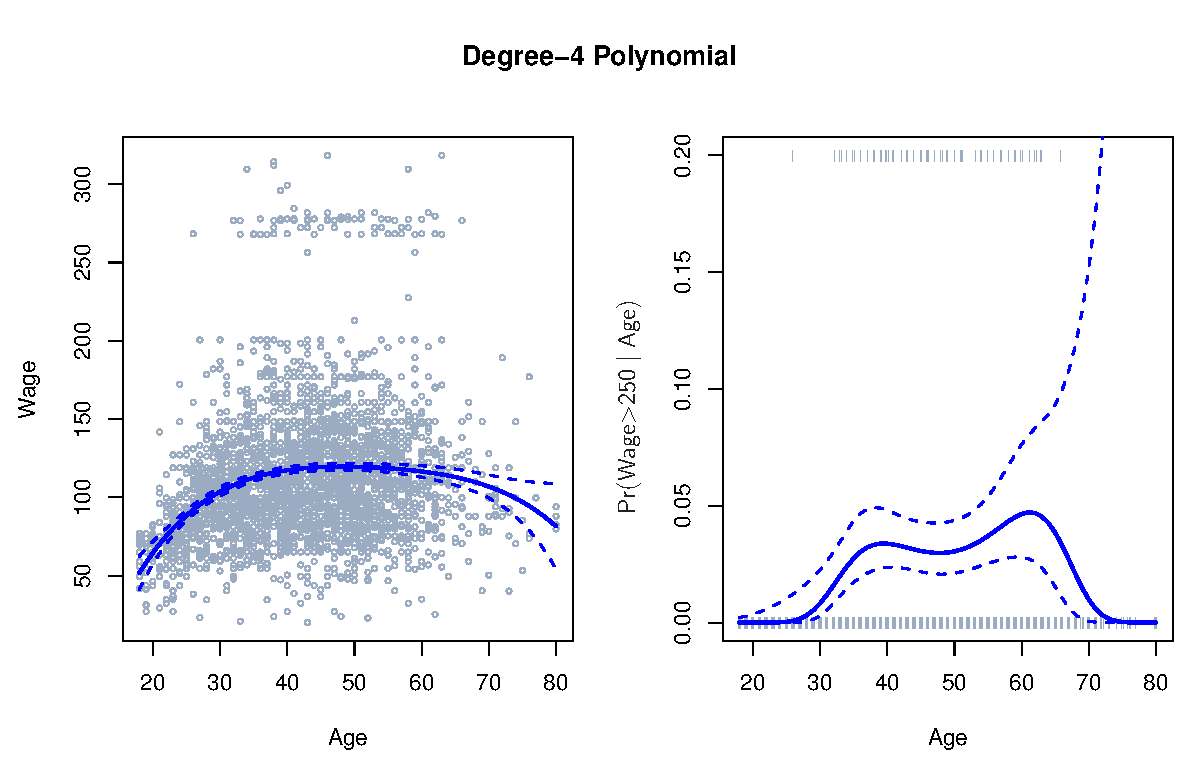
\includegraphics[width=0.92\textwidth,height=0.50\textheight,keepaspectratio]{7_1.pdf}
  \end{center}
  \begin{takeaway}Left: the degree-4 fit with its pointwise band; right: the fitted $\Pr(\text{wage}>250\mid\text{age})$. The curve captures the rise-then-plateau, but bends and widens at the sparse upper edge.\end{takeaway}
  \islpsource{Figure 7.1}
\end{frame}

\begin{frame}{Step functions: piecewise constant}
  An alternative when the relationship is naturally piecewise
  constant.
  \begin{block}{Model}
    Bin $X$ into $K+1$ ranges and fit a constant in each:
    \[
      Y = \beta_0 + \beta_1 \mathbf{1}\{c_1 \le X < c_2\} + \cdots
          + \beta_K \mathbf{1}\{c_K \le X\} + \varepsilon.
    \]
  \end{block}
  \begin{readme}[Pros and cons]
    Easy to interpret (``income bracket''), but discontinuous at the
    breakpoints --- often visually ugly. Useful when natural categories
    exist (age groups, salary tiers).
  \end{readme}
\end{frame}

\begin{frame}{Step function fit on Wage}
  \begin{center}
    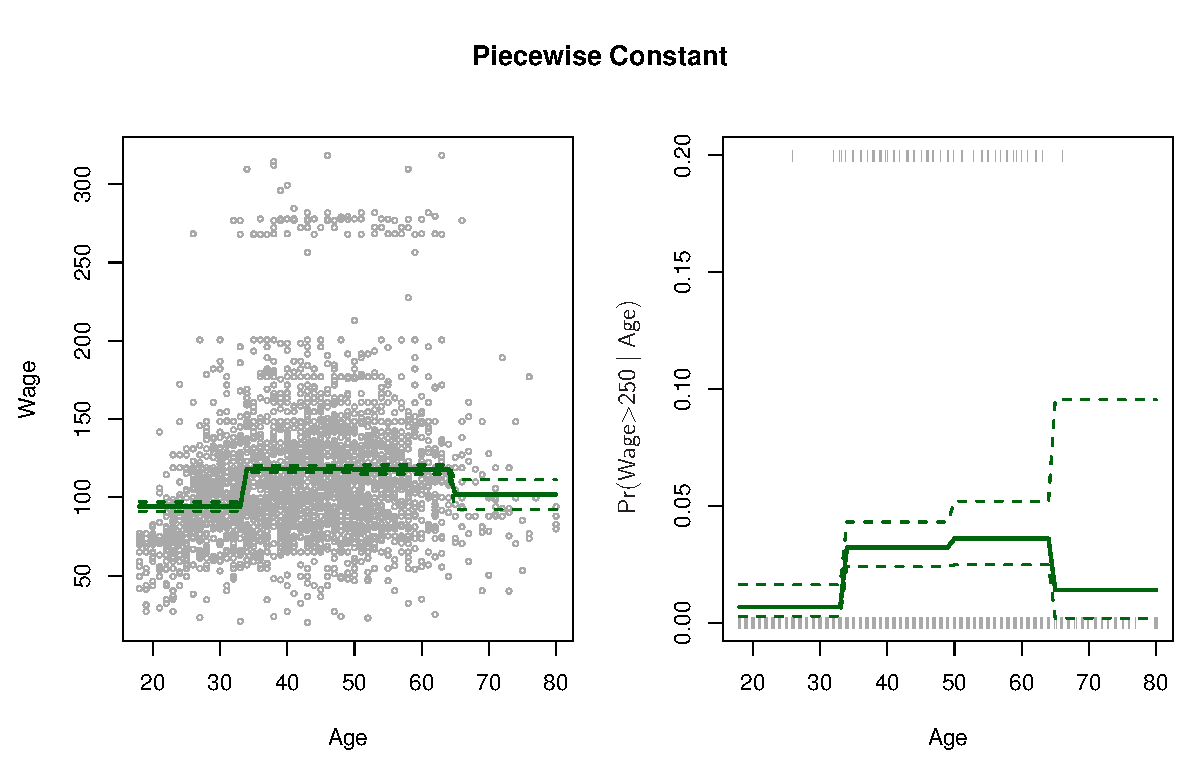
\includegraphics[width=0.92\textwidth,height=0.50\textheight,keepaspectratio]{7_2.pdf}
  \end{center}
  \begin{takeaway}Piecewise-constant: flat within each band, jumping at every cutpoint. The level shifts are captured, but the discontinuities are an artefact of binning.\end{takeaway}
  \islpsource{Figure 7.2}
\end{frame}

% ====================== EXERCISES: Polynomials ======================
\begin{frame}{Exercise 7.1 --- Evaluating a fitted cubic [Math]}
\begin{exercise}
Consider a cubic polynomial regression of \texttt{wage} on \texttt{age} using the raw basis $\{1,x,x^2,x^3\}$.
\begin{enumerate}
  \item Write the design-matrix row for a single observation with $x=2$.
  \item The fitted model is $\hat f(x)=50+4x-0.5x^2+0.1x^3$. Predict the response at $x=2$ and $x=4$.
  \item Degree three sounds nonlinear. Explain why this is still a \emph{linear} model.
\end{enumerate}
\end{exercise}
\end{frame}

\begin{frame}{Solution --- Exercise 7.1 (1/2)}
\begin{solutionbox}
\textbf{(a) Design-matrix row.} Polynomial regression is ordinary OLS on a design matrix whose columns are powers of $x$, so each observation contributes the row of its basis values. With basis $\{1,x,x^2,x^3\}$ and $x=2$:
\[ \big[\,1,\ 2,\ 2^2,\ 2^3\,\big]=\big[\,1,\ 2,\ 4,\ 8\,\big]. \]
For $n$ observations the full design matrix stacks such rows: $X_{i\cdot}=[1,\ x_i,\ x_i^2,\ x_i^3]$.

\medskip
\textbf{(b) Predict by substituting term by term} into $\hat f(x)=50+4x-0.5x^2+0.1x^3$:
\[ \hat f(2)=50+4(2)-0.5(4)+0.1(8)=50+8-2+0.8=56.8, \]
\[ \hat f(4)=50+4(4)-0.5(16)+0.1(64)=50+16-8+6.4=64.4. \]
\emph{Interpretation:} between $x=2$ and $x=4$ the prediction rises by $64.4-56.8=7.6$; the curve still climbs here, but the negative $x^2$ term is already damping the growth.
\end{solutionbox}
\end{frame}

\begin{frame}{Solution --- Exercise 7.1 (2/2)}
\begin{solutionbox}
\textbf{(c) Why this is still a linear model.} ``Linear'' refers to the \emph{coefficients}, not to the shape of the fitted curve. Writing
\[ \hat f(x)=\beta_0\cdot 1+\beta_1\cdot x+\beta_2\cdot x^2+\beta_3\cdot x^3, \]
we see $\hat f$ is a linear combination of \emph{known, pre-computed} regressors $1,x,x^2,x^3$. Hence all of the OLS machinery applies unchanged: closed-form $\hat\beta$, standard errors, $t$- and $F$-tests, cross-validation. The nonlinearity lives in $x$, not in the parameters.

\medskip
\emph{Interpretation:} this is the basis-function idea behind the whole chapter --- keep the linear-regression machinery, change only the columns of the design matrix.

\medskip
\textit{Common mistake:} predicting $\hat f(4)$ by doubling $\hat f(2)$. Polynomial predictions do not scale linearly in $x$; every power term must be substituted separately.
\end{solutionbox}
\end{frame}

\begin{frame}{Exercise 7.2 --- Step functions and dummy coding [Concept]}
\begin{exercise}
We fit a piecewise-constant (step-function) regression of \texttt{wage} on \texttt{age} using cutpoints at $35$ and $50$, giving three bins: $(-\infty,35)$, $[35,50)$, $[50,\infty)$.
\begin{enumerate}
  \item How many dummy variables do we create, and why is one bin omitted?
  \item Write the fitted model with an intercept.
  \item With $\hat\beta_0=40$, $\hat\beta_1=15$ (bin $[35,50)$), $\hat\beta_2=25$ (bin $[50,\infty)$), predict \texttt{wage} for ages $30$, $40$, and $60$.
  \item State one limitation of this approach.
\end{enumerate}
\end{exercise}
\end{frame}

\begin{frame}{Solution --- Exercise 7.2 (1/2)}
\begin{solutionbox}
\textbf{(a) Two dummies for three bins.} Define $C_1(x)=\mathbf{1}[35\le x<50]$ and $C_2(x)=\mathbf{1}[x\ge 50]$. The first bin $(-\infty,35)$ is the \emph{reference category}, absorbed into the intercept. \emph{Why omit one bin?} With an intercept, the column of ones equals the sum of all three bin dummies, so including all three would make the design matrix perfectly collinear --- the ``dummy-variable trap''. In general: $m$ bins $\Rightarrow$ $m-1$ dummies plus an intercept.

\medskip
\textbf{(b) Fitted model.}
\[ y=\beta_0+\beta_1 C_1(x)+\beta_2 C_2(x)+\varepsilon. \]
\emph{Reading the coefficients:} $\beta_0$ is the mean wage in the reference bin; $\beta_1$ and $\beta_2$ are the mean \emph{differences} of bins $2$ and $3$ relative to that reference --- not relative to each other.
\end{solutionbox}
\end{frame}

\begin{frame}{Solution --- Exercise 7.2 (2/2)}
\begin{solutionbox}
\textbf{(c) Predictions.} Locate each age's bin, switch on its dummy, and add:
\begin{itemize}
  \item Age $30<35$: reference bin, $C_1=C_2=0\Rightarrow \hat y=40$.
  \item Age $40\in[35,50)$: $C_1=1,C_2=0\Rightarrow \hat y=40+15=55$.
  \item Age $60\ge50$: $C_1=0,C_2=1\Rightarrow \hat y=40+25=65$.
\end{itemize}
\emph{Interpretation:} predicted wage steps from $40$ to $55$ at age $35$ and to $65$ at age $50$ --- everyone inside a bin gets the same prediction.

\medskip
\textbf{(d) Limitation.} The fit is constant within each bin and jumps at the cutpoints: it ignores any trend inside a bin, and the cutpoints are chosen arbitrarily. Unless the true relationship really has breakpoints, this misses smooth structure.

\medskip
\textit{Common mistake:} reading $\beta_2=25$ as the jump from bin $2$ to bin $3$. Both coefficients compare to the \emph{reference} bin; the bin-$2$-to-bin-$3$ step is $\beta_2-\beta_1=10$.
\end{solutionbox}
\end{frame}



% ============================================================
\section{Splines}
% ============================================================

\begin{frame}{Basis functions: a unifying view}
  Polynomials and step functions are special cases of:
  \begin{block}{Basis-function regression}
    \[
      Y = \beta_0 + \sum_{j=1}^K \beta_j b_j(X) + \varepsilon,
    \]
    for fixed basis functions $b_1, \ldots, b_K$.
  \end{block}
  \begin{readme}
    Read it as: each $b_j(\cdot)$ is a \emph{fixed} transformation
    chosen in advance, and $\beta_j$ is its ordinary regression weight
    --- so once the $b_j$ are set, this is plain OLS. Special cases:
    \begin{itemize}
      \item Polynomials: $b_j(X) = X^j$.
      \item Step functions: $b_j(X) = \mathbf{1}\{c_j \le X < c_{j+1}\}$.
      \item Splines: piecewise polynomials joined smoothly at chosen
            knots.
    \end{itemize}
  \end{readme}
\end{frame}

\begin{frame}{Regression splines: idea}
  Splines combine the flexibility of polynomials with the locality of
  step functions.
  \begin{block}{Construction}
    Split the range of $X$ at $K$ \emph{knots}
    $\xi_1 < \cdots < \xi_K$. Fit a polynomial of degree $d$ on each
    piece, joined at the knots so the function and its first $d-1$
    derivatives are continuous.
  \end{block}
  \begin{takeaway}[Practical defaults]
    \textbf{Cubic splines} ($d = 3$) are the standard choice --- they
    are smooth visually. Total degrees of freedom: $K + d + 1$.
  \end{takeaway}
\end{frame}

\begin{frame}{Why the continuity constraints? Broken vs.\ smooth joins}
  \begin{center}
  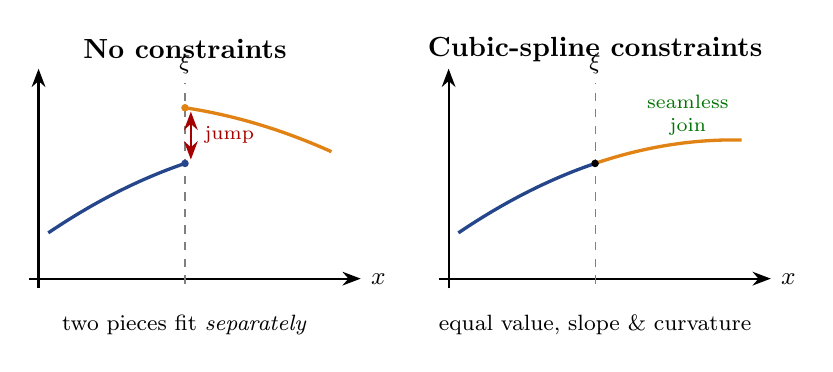
\begin{tikzpicture}[scale=0.62,>=Stealth,font=\small]
    \definecolor{cL}{RGB}{38,70,140}\definecolor{cR}{RGB}{224,130,20}
    % ---------- LEFT: no constraints ----------
    \begin{scope}
      \node[font=\bfseries] at (3,4.7) {No constraints};
      \draw[->,thick] (-0.2,0)--(6.6,0) node[right]{$x$};
      \draw[->,thick] (0,-0.2)--(0,4.3);
      \draw[gray,dashed] (3,-0.1)--(3,4.0) node[above,black,font=\footnotesize]{$\xi$};
      \draw[cL,very thick,domain=0.2:3,smooth,samples=50] plot(\x,{0.8+0.7*\x-0.06*\x*\x});
      \draw[cR,very thick,domain=3:6,smooth,samples=50] plot(\x,{3.5-0.15*(\x-3)-0.05*(\x-3)*(\x-3)});
      \fill[cL] (3,2.36) circle(2.2pt);
      \fill[cR] (3,3.5) circle(2.2pt);
      \draw[<->,red!65!black,thick] (3.12,2.44)--(3.12,3.42);
      \node[red!65!black,font=\scriptsize,right] at (3.2,2.95) {jump};
      \node[align=center,font=\footnotesize] at (3,-0.95) {two pieces fit \emph{separately}};
    \end{scope}
    % ---------- RIGHT: cubic-spline constraints ----------
    \begin{scope}[xshift=8.4cm]
      \node[font=\bfseries] at (3,4.7) {Cubic-spline constraints};
      \draw[->,thick] (-0.2,0)--(6.6,0) node[right]{$x$};
      \draw[->,thick] (0,-0.2)--(0,4.3);
      \draw[gray,dashed] (3,-0.1)--(3,4.0) node[above,black,font=\footnotesize]{$\xi$};
      \draw[cL,very thick,domain=0.2:3,smooth,samples=50] plot(\x,{0.8+0.7*\x-0.06*\x*\x});
      \draw[cR,very thick,domain=3:6,smooth,samples=50] plot(\x,{2.36+0.34*(\x-3)-0.06*(\x-3)*(\x-3)});
      \fill[black] (3,2.36) circle(2.2pt);
      \node[green!45!black,font=\scriptsize,align=center] at (4.9,3.35) {seamless\\ join};
      \node[align=center,font=\footnotesize] at (3,-0.95) {equal value, slope \& curvature};
    \end{scope}
  \end{tikzpicture}
  \end{center}
  \begin{takeaway}A regression spline is \emph{not} one global polynomial: it is separate low-degree pieces. All the work is in the join --- forcing equal value, slope and curvature at each knot makes the seam invisible while each piece stays flexible.\end{takeaway}
\end{frame}

\begin{frame}{How a cubic spline is built: continuity at the knots}
  \begin{center}
  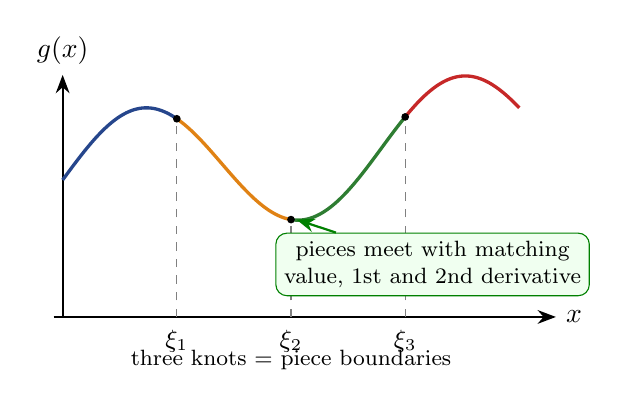
\begin{tikzpicture}[scale=0.58,>=Stealth]
    \definecolor{cA}{RGB}{38,70,140}\definecolor{cB}{RGB}{224,130,20}
    \definecolor{cC}{RGB}{46,125,50}\definecolor{cD}{RGB}{198,40,40}
    % axes
    \draw[->,thick] (-0.2,0) -- (10.8,0) node[right]{$x$};
    \draw[->,thick] (0,0) -- (0,5.3) node[above]{$g(x)$};
    % four cubic pieces of ONE smooth spline (same function => value/slope/curvature match)
    \draw[cA,very thick,domain=0:2.5,smooth,samples=60]   plot(\x,{3+1.4*sin((0.9*\x) r)+0.1*\x});
    \draw[cB,very thick,domain=2.5:5,smooth,samples=60]   plot(\x,{3+1.4*sin((0.9*\x) r)+0.1*\x});
    \draw[cC,very thick,domain=5:7.5,smooth,samples=60]   plot(\x,{3+1.4*sin((0.9*\x) r)+0.1*\x});
    \draw[cD,very thick,domain=7.5:10,smooth,samples=60]  plot(\x,{3+1.4*sin((0.9*\x) r)+0.1*\x});
    % knots
    \foreach \k/\lab in {2.5/$\xi_1$,5/$\xi_2$,7.5/$\xi_3$}{
       \pgfmathsetmacro{\yk}{3+1.4*sin((0.9*\k) r)+0.1*\k}
       \draw[gray,dashed] (\k,0) -- (\k,\yk);
       \fill[black] (\k,\yk) circle (2.4pt);
       \node[below,font=\small] at (\k,-0.08) {\lab};
    }
    \node[font=\footnotesize] at (5,-0.95) {three knots = piece boundaries};
    % annotation to middle join
    \pgfmathsetmacro{\yb}{3+1.4*sin((0.9*5) r)+0.1*5}
    \node[align=center,fill=green!6,draw=green!50!black,rounded corners,inner sep=3pt,font=\footnotesize]
       (ann) at (8.1,1.15) {pieces meet with matching\\ value, 1st and 2nd derivative};
    \draw[->,green!50!black,thick] (ann) -- (5.12,\yb);
  \end{tikzpicture}
  \end{center}
  \begin{takeaway}Each region is a free cubic, yet at every knot the pieces share value, slope and curvature --- so the joins are invisible.\end{takeaway}
\end{frame}



\begin{frame}{The natural-spline boundary fix}
  \begin{alertblock}{Boundary problem}
    Cubic splines flare beyond extreme knots. The CIs at the
    boundaries become unreliably wide.
  \end{alertblock}
  \begin{readme}[Why the edges misbehave]
    Past the outermost knots the fit is still a free cubic, but almost
    no data pin it down there. A cubic can curve sharply, so a small
    change in a boundary point swings the whole tail --- inflating
    variance exactly where evidence is thinnest.
  \end{readme}
  \begin{takeaway}[Natural cubic splines]
    Constrain the spline to be \emph{linear} past the boundary knots.
    The resulting fits are stable at the edges with negligible bias
    inside.
  \end{takeaway}
\end{frame}

\begin{frame}{Choosing knots and degrees of freedom}
  \begin{block}{Two practical decisions}
    \begin{itemize}
      \item \textbf{How many knots?} Choose by cross-validation.
            Modest df (4--8) usually suffices.
      \item \textbf{Where?} Equal quantiles of $X$ usually work well.
            With small $n$, place knots manually at obvious
            change-points.
    \end{itemize}
  \end{block}
  \begin{readme}[Why cubic and not quintic?]
    Cubic is the lowest degree that gives visually smooth fits
    (matches second derivative). Higher degrees rarely improve the
    fit but add parameters and instability.
  \end{readme}
\end{frame}

\begin{frame}{Cubic vs.\ natural spline on Wage}
  \begin{center}
    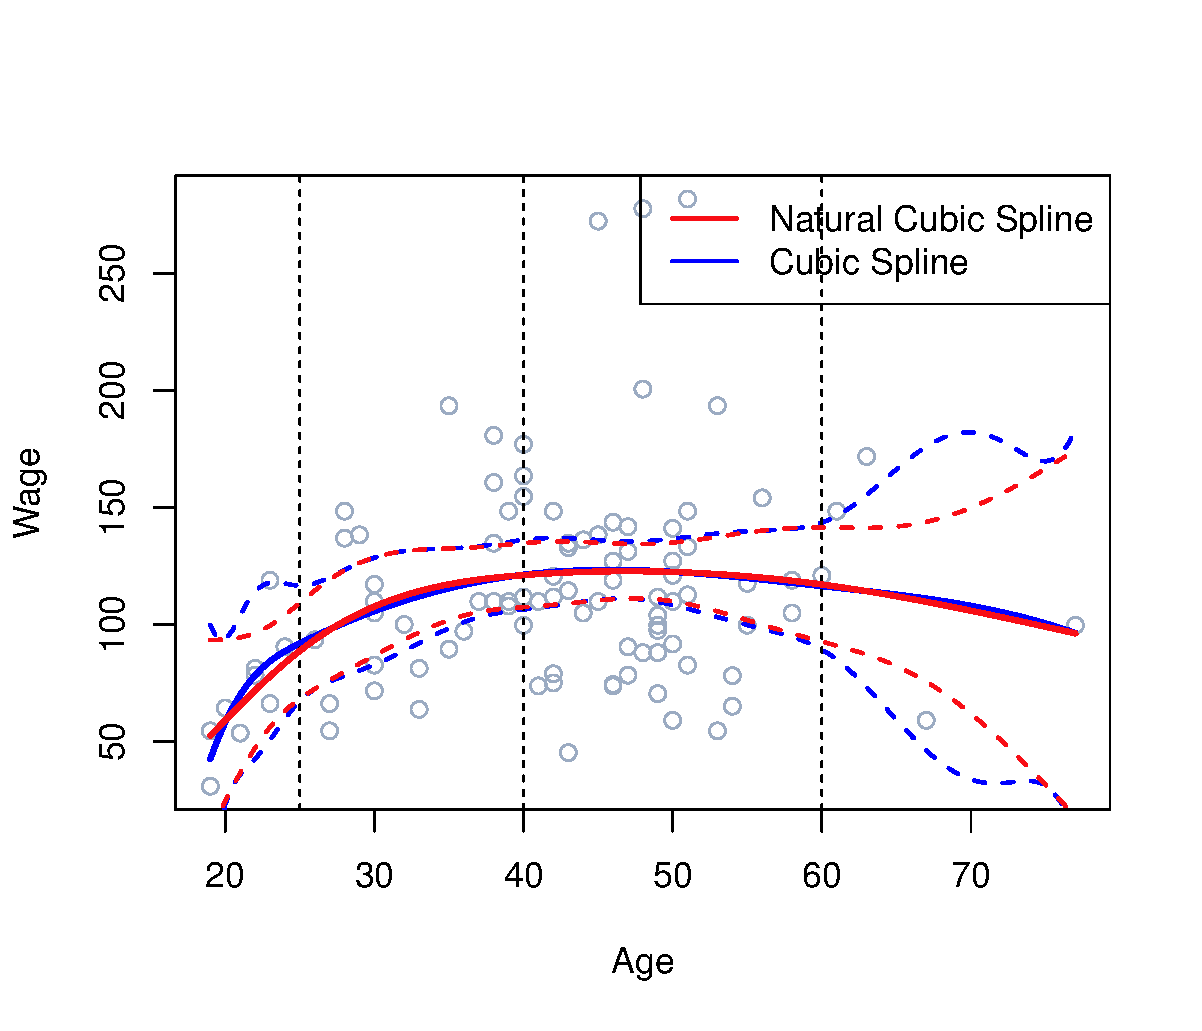
\includegraphics[width=0.85\textwidth,height=0.50\textheight,keepaspectratio]{7_4.pdf}
  \end{center}
  \begin{takeaway}Same data, two fits: the cubic spline's error bands blow up at the edges while the natural spline's stay controlled --- boundary behaviour is the deciding difference.\end{takeaway}
  \islpsource{Figure 7.4}
\end{frame}

\begin{frame}{Wage vs.\ age: four models side by side}
  \begin{center}
    
\includegraphics[width=0.86\textwidth,height=0.60\textheight,keepaspectratio]{ch07_wage_fits.png}
  \end{center}
  \begin{takeaway}All four recover the same rise--plateau--fall shape but differ at the edges: the polynomial dips, the step function is blocky, the natural spline stays smooth and stable.\end{takeaway}
\end{frame}

% ====================== EXERCISES: Splines ======================
\begin{frame}{Exercise 7.3 --- Degrees of freedom of a cubic spline [Math]}
\begin{exercise}
Consider a cubic regression spline with $K$ interior knots, fitted so that the function and its first two derivatives are continuous at each knot.
\begin{enumerate}
  \item If we fit a \emph{separate} cubic in each of the $K+1$ regions, how many free parameters is that?
  \item How many constraints do the continuity conditions impose in total?
  \item Show that the net degrees of freedom equal $K+4$.
  \item How many basis functions does the truncated-power basis use (including the intercept)? Confirm consistency.
\end{enumerate}
\end{exercise}
\end{frame}

\begin{frame}{Solution --- Exercise 7.3 (1/2)}
\begin{solutionbox}
\textbf{(a) Free parameters.} $K$ knots split the line into $K+1$ regions. Each region carries its own cubic $a_j+b_jx+c_jx^2+d_jx^3$, i.e.\ $4$ coefficients, so fitting them separately costs
\[ 4\times(K+1)=4K+4 \text{ parameters.} \]

\medskip
\textbf{(b) Constraints.} At each interior knot we require the two adjacent pieces to agree in \emph{value}, \emph{slope}, and \emph{curvature} ($g,g',g''$ continuous): $3$ constraints per knot, hence
\[ 3\times K = 3K \text{ constraints in total.} \]
\emph{Why stop at the second derivative?} Matching $g'''$ as well would force adjacent cubics to be identical --- the ``spline'' would collapse to one global cubic. Continuity up to $g''$ is exactly what the eye perceives as smooth.
\end{solutionbox}
\end{frame}

\begin{frame}{Solution --- Exercise 7.3 (2/2)}
\begin{solutionbox}
\textbf{(c) Net degrees of freedom.} Each independent linear constraint removes one free parameter:
\[ \underbrace{(4K+4)}_{\text{free params}}-\underbrace{3K}_{\text{constraints}} = K+4. \]
\emph{Sanity check:} $K=0$ gives $4$ --- a single cubic, as it must. Each additional knot buys exactly \emph{one} extra degree of freedom.

\medskip
\textbf{(d) Basis count.} The truncated-power basis is
\[ 1,\ x,\ x^2,\ x^3,\ (x-\xi_1)^3_+,\dots,(x-\xi_K)^3_+, \]
which is $4+K$ functions --- one regression coefficient each, exactly matching the $K+4$ df from (c). Each truncated term adds one knot while preserving continuity of $g,g',g''$, so the two counting arguments agree.

\medskip
\textit{Common mistake:} counting $4$ constraints per knot (including $g'''$) or forgetting the intercept among the basis functions --- both break the $K+4$ tally.
\end{solutionbox}
\end{frame}

\begin{frame}{Exercise 7.4 --- Natural vs.\ cubic splines [Concept]}
\begin{exercise}
\begin{enumerate}
  \item What extra constraints turn a cubic spline into a \emph{natural} cubic spline?
  \item A cubic spline with $K$ knots has $K+4$ df. How many df does a natural cubic spline with $K$ knots have?
  \item Why do natural splines behave better near the boundaries of the data?
  \item What does this imply for the width of pointwise confidence bands at the extremes of $x$?
\end{enumerate}
\end{exercise}
\end{frame}

\begin{frame}{Solution --- Exercise 7.4 (1/2)}
\begin{solutionbox}
\textbf{(a) Extra constraints.} A natural spline is required to be \emph{linear} beyond the two boundary knots. A function is linear exactly when its second and third derivatives vanish, so the requirement translates into
\[ g''(\xi)=0 \quad\text{and}\quad g'''(\xi)=0 \quad \text{at and beyond each boundary knot}, \]
i.e.\ $2$ extra constraints at each of the $2$ boundaries: $4$ additional constraints in total.

\medskip
\textbf{(b) Degrees of freedom.} Start from the cubic-spline count and subtract one df per constraint:
\[ (K+4)-4 = K. \]
\emph{Interpretation:} a natural spline with $K$ knots is exactly as complex as a linear model with $K$ coefficients --- its flexibility budget is spent entirely in the interior, where the data live.
\end{solutionbox}
\end{frame}

\begin{frame}{Solution --- Exercise 7.4 (2/2)}
\begin{solutionbox}
\textbf{(c) Why natural splines behave at the boundaries.} Past the outer knots an unrestricted cubic spline is still a free cubic, but almost no data pin it down there: a handful of extreme observations steer four polynomial coefficients, so small data changes swing the whole tail --- high variance exactly where evidence is thinnest. Forcing linear tails removes those unsupported cubic wiggles.

\medskip
\textbf{(d) Consequence for confidence bands.} The pointwise band width tracks the variance of $\hat g(x)$. Because fewer parameters are spent at the extremes and the tail shape is constrained to be linear, natural-spline bands are substantially \emph{narrower} at the boundaries than cubic-spline bands, at the price of a negligible bias increase in the interior.

\medskip
\textit{Common mistake:} thinking the natural spline is linear \emph{between} the boundary knots too --- inside the boundary knots it is every bit as flexible a cubic spline; only the two tails are straightened.
\end{solutionbox}
\end{frame}







% ============================================================
\section{Smoothing}
% ============================================================

\begin{frame}{Smoothing splines: let the data choose}
  Instead of choosing knots manually, place a knot at \emph{every}
  data point and let a penalty control smoothness.
  \begin{block}{Penalised RSS}
    \[
      \boxed{\;
        \min_{g} \sum_{i=1}^n (y_i - g(x_i))^2 +
        \lambda \int g''(t)^2\,dt.
      \;}
    \]
  \end{block}
\end{frame}

\begin{frame}{Reading the smoothing-spline objective}
  \begin{readme}
    \begin{tabular}{@{}cl@{}}
      \toprule
      \textbf{Term} & \textbf{Role} \\
      \midrule
      $\sum (y_i - g(x_i))^2$ & Training fit \\
      $\int g''(t)^2 dt$ & Penalty for ``wiggliness'' (curvature) \\
      $\lambda$ & Smoothness tuning parameter \\
      \bottomrule
    \end{tabular}
  \end{readme}
  \begin{takeaway}[Three observations]
    \begin{itemize}
      \item The minimiser is a natural cubic spline with knots at every
            $x_i$.
      \item $\lambda = 0$: interpolation. $\lambda \to \infty$: linear fit.
      \item ``Effective degrees of freedom'' parameterise the
            smoothness.
    \end{itemize}
  \end{takeaway}
\end{frame}

\begin{frame}{Smoothing spline on Wage}
  \begin{center}
    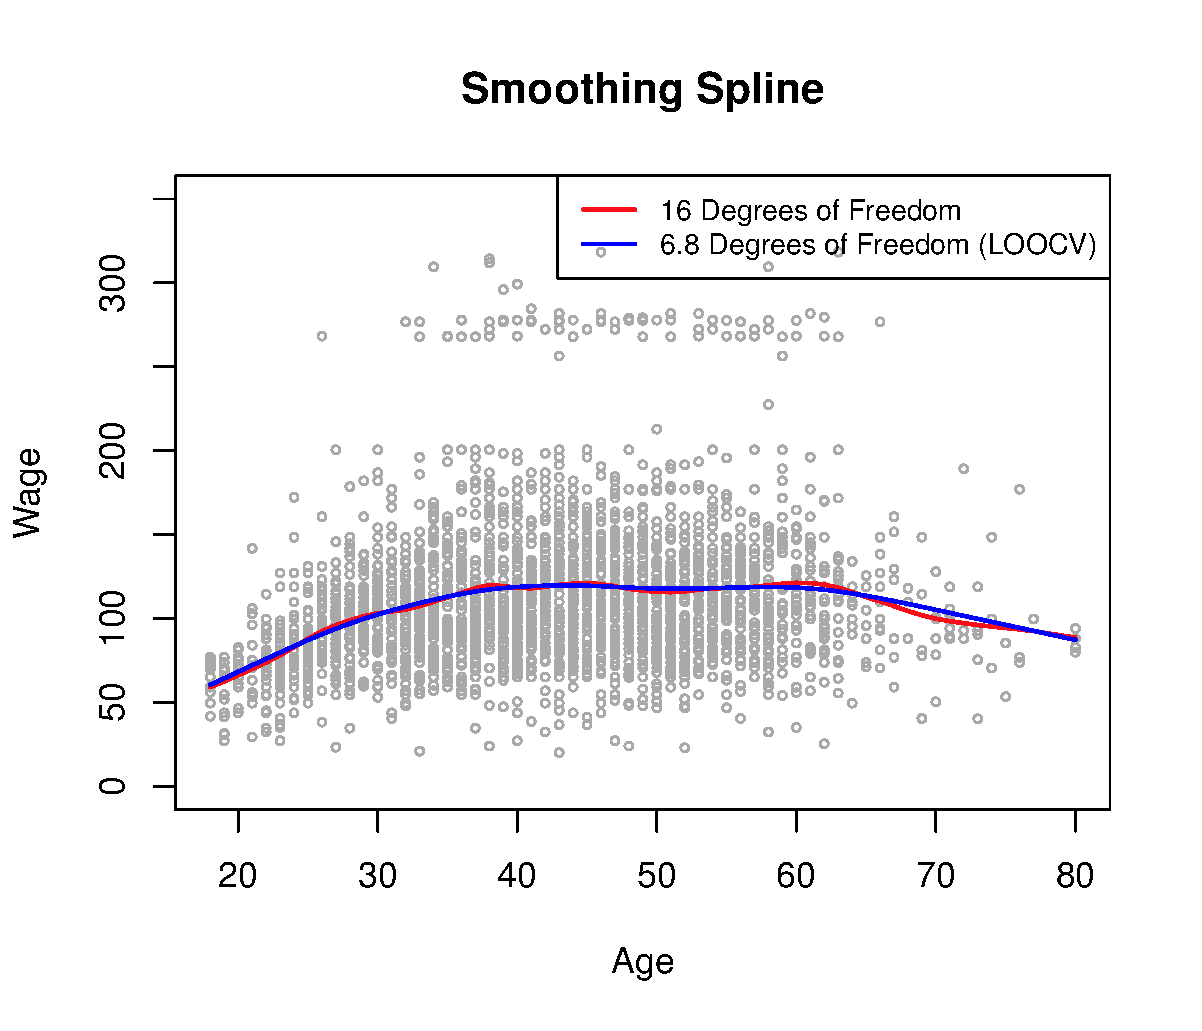
\includegraphics[width=0.85\textwidth,height=0.50\textheight,keepaspectratio]{7_8.pdf}
  \end{center}
  \begin{takeaway}Two ways to fix smoothness: a preset $16$ df vs.\ the $\approx6.8$ effective df chosen by CV. More effective df means a wigglier fit; CV finds the sweet spot.\end{takeaway}
  \islpsource{Figure 7.8}
\end{frame}

\begin{frame}{Smoothing spline flexibility: $\lambda$ is the dial}
  \begin{center}
\includegraphics[width=0.88\textwidth,height=0.50\textheight,keepaspectratio]{ch07_x_smooth_spline.png}\end{center}
  \begin{takeaway}Same Wage data, two penalties: $\lambda=10^4$ gives a calm trend ($\approx 3.7$ effective df) while $\lambda=0.1$ ($\approx 43$ df) chases noise --- $\lambda$ is the flexibility dial, tuned by CV/LOOCV.\end{takeaway}
\end{frame}

\begin{frame}{Local regression (LOESS): a different philosophy}
  Instead of one global function, fit a small model around each point.
  \begin{block}{Recipe at each query point $x_0$}
    \begin{enumerate}
      \item Find the fraction $s$ (``span'') of points closest to
            $x_0$.
      \item Weight them by a kernel that decays with distance.
      \item Fit a low-degree polynomial by weighted least squares.
      \item Evaluate at $x_0$; repeat over the grid of $x_0$.
    \end{enumerate}
  \end{block}
  \begin{readme}
    Span $s$ controls smoothness --- the analogue of $\lambda$. LOESS
    is excellent for one or two predictors and dies fast as $p$ grows.
  \end{readme}
\end{frame}

\begin{frame}{LOESS on Wage}
  \begin{center}
    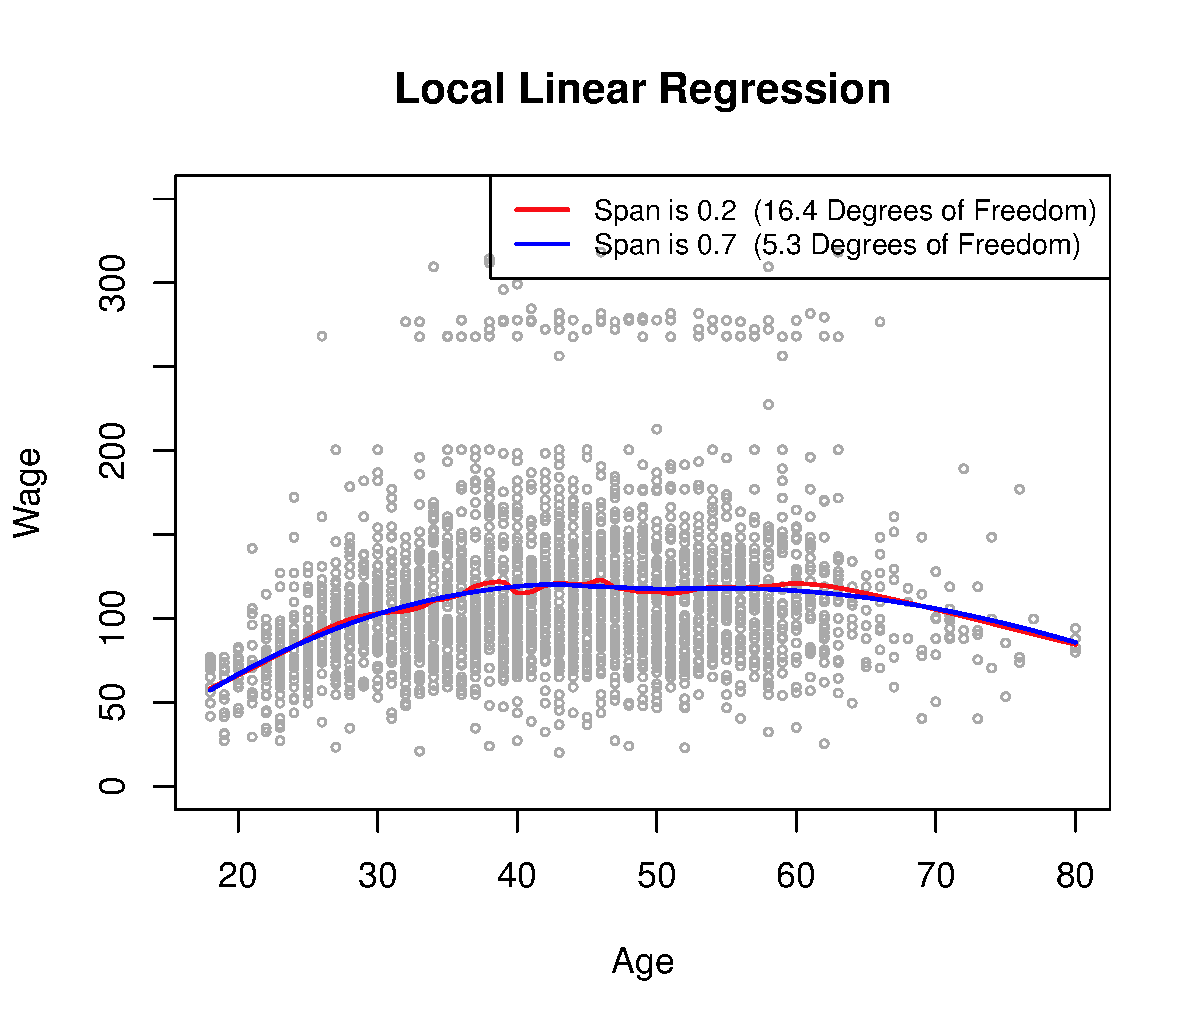
\includegraphics[width=0.85\textwidth,height=0.50\textheight,keepaspectratio]{7_10.pdf}
  \end{center}
  \begin{takeaway}Each curve uses a different span: $0.2$ tracks local wiggles, $0.7$ is smoother. Span plays the role of $\lambda$, trading bias against variance.\end{takeaway}
  \islpsource{Figure 7.10}
\end{frame}


\begin{frame}{Mini-check: spline choices}
  \begin{readme}[Quick self-assessment]
    \begin{enumerate}
      \item Why prefer a natural cubic spline over a regular cubic
            spline at the boundaries?
      \item How is a smoothing spline's $\lambda$ related to its
            effective degrees of freedom?
      \item In LOESS, what happens to bias as the span shrinks?
    \end{enumerate}
  \end{readme}
  \begin{takeaway}[Answers]
    1.\ Natural splines are constrained linear past the boundary knots,
        avoiding wild boundary oscillation.\quad
    2.\ Larger $\lambda$ $\Rightarrow$ smaller df (more shrinkage,
        smoother fit).\quad
    3.\ Bias decreases (the local fit is more local), but variance
        increases.
  \end{takeaway}
\end{frame}

% ====================== EXERCISE: Smoothing ======================
\begin{frame}{Exercise 7.5 --- Smoothing splines and $\lambda$ [Concept]}
\begin{exercise}
A smoothing spline chooses $g$ to minimise
\[ \sum_{i=1}^n (y_i-g(x_i))^2 \;+\; \lambda\!\int g''(t)^2\,dt. \]
\begin{enumerate}
  \item Interpret the penalty term. What does it measure?
  \item Describe the fit as $\lambda\to 0$ and as $\lambda\to\infty$.
  \item Define the effective degrees of freedom $\mathrm{df}_\lambda$ and give its range.
  \item How is $\lambda$ chosen in practice?
\end{enumerate}
\end{exercise}
\end{frame}

\begin{frame}{Solution --- Exercise 7.5 (1/2)}
\begin{solutionbox}
\textbf{(a) The penalty measures curvature.} $g''(t)$ is the rate of change of the slope at $t$; squaring removes the sign and integrating adds curvature up over the whole range, so $\int g''(t)^2\,dt$ is the total \emph{roughness} of $g$. A straight line has $g''\equiv0$ and pays no penalty; a wiggly curve pays a lot. The penalty therefore discourages wiggliness.

\medskip
\textbf{(b) The two extremes.} As $\lambda\to 0$ curvature becomes free, so the minimiser drives the RSS term to $0$: $g$ \emph{interpolates} the data --- extremely wiggly, low bias, high variance. As $\lambda\to\infty$ any curvature is infinitely expensive, forcing $g''=0$ everywhere, so $g$ collapses to the ordinary least-squares \emph{line}.

\medskip
\emph{Interpretation:} $\lambda$ sweeps a continuous bridge between interpolation and linear regression --- it is the bias--variance dial of the smoothing spline.
\end{solutionbox}
\end{frame}

\begin{frame}{Solution --- Exercise 7.5 (2/2)}
\begin{solutionbox}
\textbf{(c) Effective degrees of freedom.} For fixed $\lambda$ the fit is linear in $y$: $\hat g=S_\lambda\,y$ for a smoother matrix $S_\lambda$. In OLS the analogous ``hat'' matrix has trace equal to the number of parameters, which motivates the definition
\[ \mathrm{df}_\lambda=\operatorname{trace}(S_\lambda), \]
ranging from $n$ (at $\lambda=0$, interpolation) down to $2$ (at $\lambda\to\infty$, slope $+$ intercept of the linear fit).

\medskip
\textbf{(d) Choosing $\lambda$.} By cross-validation. LOOCV is essentially free because each leave-one-out residual follows from the \emph{single} full fit via the leverage $\{S_\lambda\}_{ii}$:
\[ \mathrm{RSS}_{\text{cv}}(\lambda)=\sum_{i=1}^n\!\left(\frac{y_i-\hat g_\lambda(x_i)}{1-\{S_\lambda\}_{ii}}\right)^{\!2}. \]

\textit{Common mistake:} picking $\lambda$ by minimising \emph{training} RSS --- that always selects $\lambda=0$ (interpolation). Only out-of-sample criteria can trade fit against roughness.
\end{solutionbox}
\end{frame}


% ============================================================
\section{GAMs}
% ============================================================

\begin{frame}{From one predictor to many: GAMs}
  Everything we have done so far is for one predictor at a time.
  Generalised additive models lift the techniques into the
  multivariate setting.
  \begin{block}{The GAM model}
    \[
      \boxed{\;
        Y = \beta_0 + \sum_{j=1}^p f_j(X_j) + \varepsilon,
      \;}
    \]
    where each $f_j$ is a smooth function (spline or LOESS).
  \end{block}
  \begin{readme}[Symbol by symbol]
    $\beta_0$ is the overall level; each $f_j$ is a smooth,
    data-driven curve for predictor $X_j$; summing them keeps the model
    additive. Setting $f_j(X_j)=\beta_j X_j$ recovers ordinary linear
    regression --- the GAM simply lets each term bend.
  \end{readme}
\end{frame}

\begin{frame}{Why GAMs are so useful}
  \begin{takeaway}[Three reasons]
    \begin{enumerate}
      \item Generalises linear regression: $f_j(X_j) = \beta_j X_j$ is
            the linear special case.
      \item Avoids the curse of dimensionality via the additive
            structure.
      \item Each $f_j$ can be plotted separately --- excellent
            interpretability.
    \end{enumerate}
  \end{takeaway}
  \begin{alertblock}{Limitation}
    By construction, GAMs miss interactions. Add tensor-product terms
    $f_{jk}(X_j, X_k)$ explicitly, or move to trees (Ch.~8).
  \end{alertblock}
\end{frame}

\begin{frame}{GAM fit on Wage}
  \begin{center}
    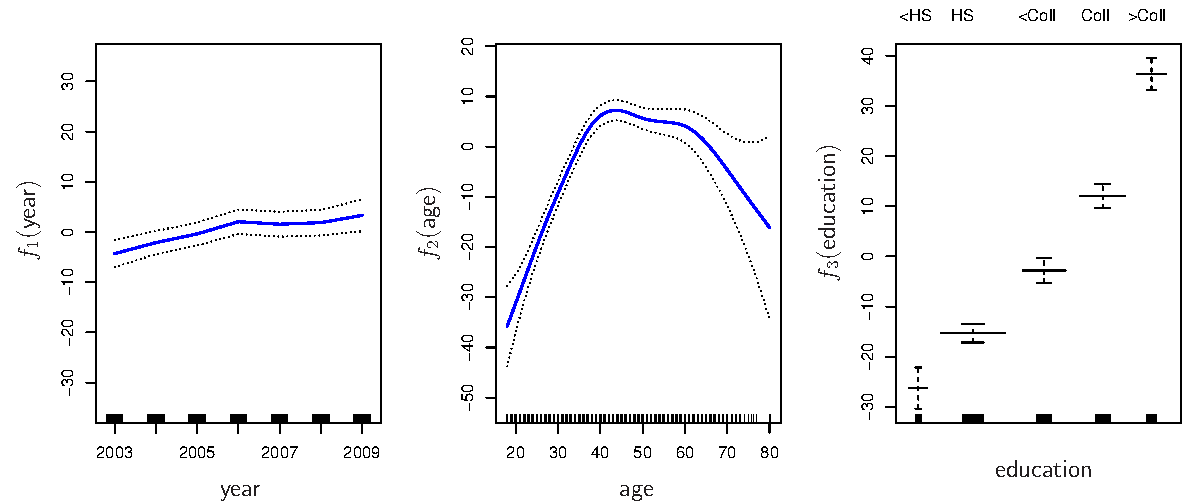
\includegraphics[width=0.95\textwidth,height=0.62\textheight,keepaspectratio]{7_12.pdf}
  \end{center}
  Each panel: estimated $f_j$ for a different predictor, with
  pointwise confidence bands.
  \islpsource{Figure 7.12}
\end{frame}

\begin{frame}{GAM component functions fitted on Wage}
  \begin{center}
    
\includegraphics[width=0.9\textwidth,height=0.58\textheight,keepaspectratio]{ch07_gam_components.png}
  \end{center}
  \begin{takeaway}Reading each partial effect: wage rises with age then falls after $\sim$60; it drifts up gently with year; and it increases monotonically with education. The additive structure lets us plot and interpret one predictor at a time.\end{takeaway}
\end{frame}

\begin{frame}{GAMs for classification}
  Same idea inside a GLM:
  \begin{block}{Logistic GAM}
    \[
      \log\frac{p(X)}{1 - p(X)} = \beta_0 + \sum_{j=1}^p f_j(X_j).
    \]
  \end{block}
  \begin{readme}[Reading the model]
    The left side is the \emph{log-odds} of the positive class; each
    smooth $f_j$ shifts those log-odds up or down as $X_j$ changes. It
    is an additive logistic model --- interpret every $f_j$ on its own,
    just as in a linear GLM.
  \end{readme}
  Combines logistic regression's interpretability with smooth
  per-predictor effects. Implementations: \texttt{pyGAM},
  \texttt{statsmodels.gam}.
\end{frame}

% ====================== EXTENDED EXERCISE: GAMs ======================
\begin{frame}{Extended Exercise 7.2 --- A GAM for wage [Integrative]}
\begin{longexercise}
Fit a generalised additive model
\[ \mathtt{wage} \approx \beta_0 + s(\mathtt{age}) + \mathtt{year} + f(\mathtt{education}), \]
with a smooth spline in \texttt{age}, a (near-)linear term in \texttt{year}, and \texttt{education} as a factor.
\begin{enumerate}
  \item Fit it (e.g.\ \texttt{pyGAM}) and state how a GAM is estimated.
  \item Interpret each partial effect.
  \item Which term is genuinely non-linear? Discuss the effective degrees of freedom (EDF) of each term.
  \item State the advantages of the additive form and its key limitation. Give an interaction it would miss and how to add it.
\end{enumerate}
\end{longexercise}
\end{frame}

\begin{frame}[fragile]{Solution --- Extended Exercise 7.2 (1/3)}
\begin{solutionbox}
\textbf{(a) Fit \& algorithm.} Encode \texttt{education} to integer codes, then fit a spline in age, a linear term in year and a factor in education:
\begin{lstlisting}
import pandas as pd
from pygam import LinearGAM, s, l, f

W = pd.read_csv('../../ALL CSV FILES - 2nd Edition/Wage.csv')  # load Wage
W['edu'] = W['education'].astype('category').cat.codes  # factor -> codes
X = W[['age', 'year', 'edu']].values  # predictor matrix
y = W['wage'].values                  # response
gam = LinearGAM(s(0) + l(1) + f(2)).fit(X, y)  # s=spline, l=linear, f=factor
gam.summary()   # effective DoF and p-value per term
\end{lstlisting}
A GAM is fit by \emph{backfitting}: cycle through the terms, repeatedly re-estimating each $f_j$ on the partial residual $y-\beta_0-\sum_{k\neq j}f_k(X_k)$ until the fit stabilises --- each smooth is refitted to whatever the other terms leave unexplained.
\end{solutionbox}
\end{frame}

\begin{frame}{Solution --- Extended Exercise 7.2 (2/3)}
\begin{solutionbox}
\textbf{(b) Partial effects} (each holds the others fixed):
\begin{itemize}
  \item \texttt{age}: a pronounced \emph{hump} --- wage climbs steeply to about age $40$, plateaus through the $50$s, then declines after $\sim$60.
  \item \texttt{year}: a gentle, near-linear \emph{increase} --- slow wage growth over the sample window.
  \item \texttt{education}: a monotone \emph{staircase} --- each higher band pays more, ``Advanced Degree'' far above ``$<$HS Grad''.
\end{itemize}

\textbf{(c) Non-linearity \& EDF.} Only \texttt{age} is genuinely non-linear: its smooth spends several effective degrees of freedom (roughly $4$--$6$). \texttt{year} enters with EDF $\approx1$ (essentially a straight line); \texttt{education} as a factor contributes df $=$ (levels $-1$) $=4$. The EDF is how a GAM quantifies ``how wiggly'' each term is.

\medskip
\textit{Common mistake:} reading a partial-effect curve as an absolute wage level. Each panel is centred around zero; only its \emph{shape} and within-panel differences are meaningful, with all other predictors held fixed.
\end{solutionbox}
\end{frame}

\begin{frame}{Solution --- Extended Exercise 7.2 (3/3)}
\begin{solutionbox}
\textbf{(d) Advantages of additivity.}
\begin{itemize}
  \item Each term is estimated and \emph{plotted separately}, so effects are directly interpretable.
  \item The additive structure sidesteps the curse of dimensionality (no $p$-dimensional smoother).
  \item It strictly generalises linear regression: a linear term is the special case $f_j(X_j)=\beta_j X_j$.
\end{itemize}

\textbf{Key limitation --- no interactions.} By construction the shape of $s(\texttt{age})$ is the \emph{same} at every education level. If the wage--age profile were steeper for college graduates than for high-school graduates (an \texttt{age}$\times$\texttt{education} interaction), the additive GAM could not represent it. \emph{Fix:} add a bivariate/tensor term $f(\texttt{age},\texttt{education})$, fit separate age-smooths per group, or move to trees / boosting (Ch.~8), which capture interactions automatically.
\end{solutionbox}
\end{frame}


% ============================================================
\section{Python Lab}

\begin{frame}{Python lab --- run it live in the notebook}
  \begin{labnote}[Companion notebook: \texttt{chapter\_07\_lab.ipynb}]
    The code in this section is meant to be \textbf{demonstrated live}. Open the companion Jupyter notebook and run it cell by cell:
    \begin{itemize}
      \item polynomial regression and step functions;
      \item regression splines and LOESS;
      \item generalised additive models (GAMs).
    \end{itemize}
    Data loads via the \texttt{ISLP} package or the bundled CSV files; the notebook ends with hands-on exercises.
  \end{labnote}
\end{frame}


% ============================================================

\begin{frame}[fragile]{Polynomial regression}
  \begin{lstlisting}
import statsmodels.api as sm
from ISLP import load_data
from ISLP.models import poly, ModelSpec as MS

Wage = load_data("Wage")  # load the Wage data
design = MS([poly("age", degree=4)]).fit_transform(Wage)  # degree-4 basis
res = sm.OLS(Wage["wage"], design).fit()  # OLS on expanded design
print(res.summary())  # coefficient table
  \end{lstlisting}
\end{frame}

\begin{frame}[fragile]{Regression splines}
  \begin{lstlisting}
from ISLP.models import bs, ns

design  = MS([bs("age", df=6)]).fit_transform(Wage)  # cubic spline, 6 df
design2 = MS([ns("age", df=4)]).fit_transform(Wage)  # natural spline, 4 df
res = sm.OLS(Wage["wage"], design2).fit()  # OLS on the spline basis
print(res.summary())  # per-basis coefficients
  \end{lstlisting}
\end{frame}

\begin{frame}[fragile]{Local regression with statsmodels}
  \begin{lstlisting}
import statsmodels.nonparametric.api as nps

l = nps.lowess(endog=Wage["wage"], exog=Wage["age"],  # local regression
               frac=0.2, return_sorted=True)  # span: 20% nearest points
import matplotlib.pyplot as plt
plt.scatter(Wage["age"], Wage["wage"], s=4, alpha=0.3)  # raw data
plt.plot(l[:, 0], l[:, 1], color="orange")  # fitted LOESS curve
plt.show()
  \end{lstlisting}
\end{frame}

\begin{frame}[fragile]{A simple GAM with pyGAM}
  \begin{lstlisting}
from pygam import LinearGAM, s, f

Wage["education"] = Wage["education"].astype("category").cat.codes  # encode factor
X = Wage[["year", "age", "education"]]  # three predictors
y = Wage["wage"]                        # response
gam = LinearGAM(s(0) + s(1) + f(2)).fit(X, y)  # smooth year, age; factor edu
gam.summary()  # EDF and p-values per term
  \end{lstlisting}
\end{frame}

% ====================== EXERCISE: Python (Wage) ======================
\begin{frame}[fragile]{Exercise 7.6 --- Natural spline / GAM on Wage [Python]}
\begin{exercise}
Using \texttt{Wage.csv}:
\begin{enumerate}
  \item Fit \texttt{wage} on a natural cubic spline of \texttt{age} with $5$ df via OLS.
  \item Fit a GAM \texttt{wage} $\sim s(\texttt{age})+s(\texttt{year})$.
  \item Describe the estimated effect of \texttt{age}.
\end{enumerate}
\end{exercise}
\end{frame}

\begin{frame}[fragile]{Solution --- Exercise 7.6 (1/3)}
\begin{solutionbox}
\textbf{(a)} Natural cubic spline via \texttt{patsy}'s \texttt{cr()} basis --- \texttt{cr()} expands \texttt{age} into $5$ natural-spline columns (linear tails built in), so the fit is still ordinary OLS:
\begin{lstlisting}
import pandas as pd
import statsmodels.formula.api as smf

Wage = pd.read_csv('../../ALL CSV FILES - 2nd Edition/Wage.csv')  # load
fit = smf.ols('wage ~ cr(age, df=5)', data=Wage).fit()  # natural spline
print(fit.summary())  # coefficient table
\end{lstlisting}
\emph{What the output shows:} $6$ coefficients (intercept $+$ $5$ basis columns), $R^2\approx0.087$, and an overall $F$-test with $p\approx10^{-56}$ --- the spline terms are jointly highly significant, even though \texttt{age} alone explains only a modest share of wage variance.
\end{solutionbox}
\end{frame}

\begin{frame}[fragile]{Solution --- Exercise 7.6 (2/3)}
\begin{solutionbox}
\textbf{(b)} A GAM with smooth terms via \texttt{pyGAM} --- each \texttt{s()} is a penalised spline whose wiggliness is measured in effective degrees of freedom (EDF):
\begin{lstlisting}
import numpy as np
from pygam import LinearGAM, s

X = Wage[['age', 'year']].values  # predictor matrix
y = Wage['wage'].values           # response
gam = LinearGAM(s(0) + s(1)).fit(X, y)  # smooth terms in age and year
gam.summary()  # EDF per smooth term
\end{lstlisting}
\emph{What the output shows:} with pyGAM's default penalty the \texttt{age} smooth uses $\approx15$ EDF and \texttt{year} $\approx6$ --- both flexible; tuning $\lambda$ by \texttt{gam.gridsearch(X, y)} shrinks the smooths toward simpler shapes. Both terms are reported significant.
\end{solutionbox}
\end{frame}

\begin{frame}{Solution --- Exercise 7.6 (3/3)}
\begin{solutionbox}
\textbf{(c)} \textit{Interpretation.} The fitted effect of \texttt{age} is clearly nonlinear: \texttt{wage} rises steeply from the late teens to about age $40$, is roughly flat (a plateau) between $40$ and $60$, then declines gently after $60$. A straight line would miss this rise-then-plateau-then-fall shape, which is why a spline / GAM is preferable. The \texttt{year} effect is mildly increasing (slow wage growth over time).

\medskip
\emph{How to read the fit:} plot \texttt{gam.partial\_dependence()} per term rather than staring at coefficients --- the spline basis coefficients have no individual meaning; only the fitted curve does.

\medskip
\textit{Common mistake:} interpreting single spline-basis coefficients (or their $t$-tests) as ``the effect of age''. Judge the term by its fitted curve and a \emph{joint} test of all its basis columns.
\end{solutionbox}
\end{frame}

% ====================== EXTENDED EXERCISE: Python (Wage) ======================
\begin{frame}{Extended Exercise 7.3 --- Three fits for wage vs.\ age [Python]}
\begin{longexercise}
Using \texttt{Wage.csv}, model \texttt{wage} as a function of \texttt{age} three ways and compare:
\begin{enumerate}
  \item a \textbf{polynomial}, choosing the degree by nested ANOVA $F$-tests (or $5$-fold CV);
  \item a \textbf{step function} (bin \texttt{age} into several ranges);
  \item a \textbf{natural cubic spline} with about $5$ df.
\end{enumerate}
Overlay the three fitted curves on a scatterplot, report the chosen complexity, and interpret where the fits agree and where they differ.
\end{longexercise}
\end{frame}

\begin{frame}[fragile]{Solution --- Extended Exercise 7.3 (1/3)}
\begin{solutionbox}
\textbf{Choose the polynomial degree by nested ANOVA.}
\begin{lstlisting}[basicstyle=\ttfamily\scriptsize]
import numpy as np, pandas as pd
import statsmodels.formula.api as smf
from statsmodels.stats.anova import anova_lm

W = pd.read_csv('../../ALL CSV FILES - 2nd Edition/Wage.csv')  # load Wage
terms = lambda d: '+'.join(f'np.power(age,{k})' for k in range(1, d+1))  # power basis
models = [smf.ols('wage ~ '+terms(d), data=W).fit() for d in range(1, 6)]  # degrees 1..5
print(anova_lm(*models)[['df_diff', 'F', 'Pr(>F)']].round(4))  # nested F-tests
\end{lstlisting}
Each row of \texttt{anova\_lm} tests degree $d$ against $d{+}1$ --- valid because the models are \emph{nested}. The $F$-tests are highly significant up to degree $3$ ($2\!\to\!3$: $p\approx0.002$), \emph{borderline} for $3\!\to\!4$ ($p\approx0.05$) and clearly insignificant for $4\!\to\!5$ ($p\approx0.37$). $5$-fold CV of test MSE is essentially flat over degrees $3$--$4$. \textbf{Chosen degree: $3$ (cubic).}
\end{solutionbox}
\end{frame}

\begin{frame}[fragile]{Solution --- Extended Exercise 7.3 (2/3)}
\begin{solutionbox}
\textbf{Step function, natural spline, and the overlay.}
\begin{lstlisting}[basicstyle=\ttfamily\scriptsize]
import matplotlib.pyplot as plt
poly = smf.ols('wage ~ '+terms(3), data=W).fit()  # cubic polynomial
W['bin'] = pd.cut(W['age'], [17,25,35,45,55,65,81])  # six age bins
step = smf.ols('wage ~ C(bin)', data=W).fit()  # step function
ns   = smf.ols('wage ~ cr(age, df=5)', data=W).fit()   # natural spline

g = pd.DataFrame({'age': np.arange(18, 81)})  # prediction grid
g['bin'] = pd.cut(g['age'], [17,25,35,45,55,65,81])  # bin grid too
plt.scatter(W['age'], W['wage'], s=4, alpha=.15, color='grey')  # data
for m, lab in [(poly,'poly (d=3)'), (step,'step'), (ns,'natural spline')]:
    plt.plot(g['age'], m.predict(g), label=lab)  # overlay each fit
plt.legend(); plt.xlabel('age'); plt.ylabel('wage'); plt.show()
\end{lstlisting}
\emph{Why the grid carries both columns:} \texttt{predict} re-applies each formula, so \texttt{g} must contain \texttt{age} (for \texttt{poly}, \texttt{ns}) \emph{and} the matching \texttt{bin} labels (for \texttt{step}), built with the \emph{same} cutpoints as in training.
\end{solutionbox}
\end{frame}

\begin{frame}{Solution --- Extended Exercise 7.3 (3/3)}
\begin{solutionbox}
\textbf{Reading the overlay.}
\begin{itemize}
  \item \emph{Where they agree:} in the data-dense interior (ages $\sim$25--70) all three fits trace the same rise--plateau--fall --- \texttt{wage} climbs steeply to about age $40$, is roughly flat through the $50$s, then eases down.
  \item \emph{Where they differ:} at the sparse boundaries. The polynomial can bend sharply at the extremes; the step function is blocky and \emph{discontinuous} at the cut-points; the natural cubic spline stays smooth and, being linear beyond its outer knots, is the most stable at the edges.
\end{itemize}
\textbf{Chosen complexity:} a cubic polynomial (degree $3$--$4$), a $6$-bin step function, and a natural spline with $\sim$5 df --- all three explain a similar share of variance ($R^2\approx0.08$--$0.09$), but the natural spline is preferred for its boundary stability.

\medskip
\textit{Common mistake:} picking the degree that maximises training $R^2$ --- it rises mechanically with every added term; only the nested $F$-tests or CV can say when the gain is real.
\end{solutionbox}
\end{frame}



% ============================================================
\section{Summary}
% ============================================================

\begin{frame}{Chapter 7 in one slide}
  \begin{block}{What we accomplished}
    A toolbox for adding flexibility to a regression while keeping the
    additive, interpretable structure of a linear model.
  \end{block}
  \begin{itemize}
    \item Polynomials, step functions, regression splines, smoothing
          splines, LOESS.
    \item GAMs as the natural multivariate extension.
    \item Cross-validation chooses the smoothness in every method.
  \end{itemize}
\end{frame}

\begin{frame}{Key formulas at a glance}
  \footnotesize
  \begin{description}
    \item[Polynomial] $y_i=\beta_0+\beta_1 x_i+\beta_2 x_i^2+\dots+\beta_d x_i^d+\varepsilon_i$.
    \item[Step function] $y_i=\beta_0+\sum_{k=1}^{K}\beta_k C_k(x_i)+\varepsilon_i$, with bins $C_k$.
    \item[Cubic spline] truncated-power basis $x,x^2,x^3,(x-\xi_k)_+^3$; \ $K$ knots $\Rightarrow$ df $=K+4$.
    \item[Natural spline] linear beyond the boundary knots; \ df $=K$.
    \item[Smoothing spline] $\min_g\ \sum_i\big(y_i-g(x_i)\big)^2+\lambda\!\int g''(t)^2\,dt$.
    \item[GAM] $y_i=\beta_0+f_1(x_{i1})+f_2(x_{i2})+\dots+f_p(x_{ip})+\varepsilon_i$.
  \end{description}
\end{frame}

\begin{frame}{Vocabulary checklist}
  \footnotesize
  \begin{tabular}{ll}
    \toprule
    \textbf{Term} & \textbf{Meaning} \\
    \midrule
    Basis function & Fixed transformation $b_j(X)$ entering linearly \\
    Knot & Breakpoint where pieces of a spline meet \\
    Cubic / natural spline & Degree-3 piecewise polynomial / linear at boundaries \\
    Smoothing spline & Penalised second-derivative fit \\
    Effective degrees of freedom & Trace of the smoother matrix \\
    LOESS / local regression & Weighted local polynomial \\
    Span & Fraction of nearest neighbours used in LOESS \\
    GAM & $Y = \beta_0 + \sum_j f_j(X_j) + \varepsilon$ \\
    Backfitting & Iterative algorithm for fitting GAMs \\
    \bottomrule
  \end{tabular}
\end{frame}

\begin{frame}{Methods comparison}
  \footnotesize
  \begin{tabular}{lll}
    \toprule
    \textbf{Method} & \textbf{Strength} & \textbf{Weakness} \\
    \midrule
    Polynomial & Easy, captures curvature & Boundary oscillation \\
    Step function & Interpretable & Discontinuous \\
    Cubic spline & Smooth, controllable df & Boundary blow-up \\
    Natural spline & Stable boundaries & Tiny extra bias inside \\
    Smoothing spline & Auto-fitting smoothness & Black-box df \\
    LOESS & Locally adaptive & Curse of dimensionality \\
    GAM & Additive, interpretable & Misses interactions unless added \\
    \bottomrule
  \end{tabular}
\end{frame}

\begin{frame}{Decision rules of thumb}
  \begin{itemize}
    \item For a single $X$ and modest curvature: polynomial degree
          2--4.
    \item For a single $X$ with multiple regimes: regression splines
          with a handful of knots placed at quantiles.
    \item For boundary stability: \emph{natural} cubic splines.
    \item For multiple predictors with little interaction: a GAM.
    \item Choose smoothness (df, $\lambda$, span) by cross-validation.
    \item For visible interactions: add tensor-product terms or move
          to trees (Ch.~8).
  \end{itemize}
\end{frame}

\begin{frame}{Common pitfalls}
  \begin{alertblock}{Don't}
    \begin{enumerate}
      \item Use polynomials of degree $> 4$ on real data.
      \item Place knots arbitrarily without checking residuals.
      \item Forget that LOESS fails fast as $p$ grows.
      \item Compare GAM df with linear-regression df one-for-one.
      \item Trust pointwise CIs of smoothing splines for inference.
      \item Ignore extrapolation --- splines outside the data range
            are unreliable.
    \end{enumerate}
  \end{alertblock}
\end{frame}

\begin{frame}{Connections to the rest of the course}
  \begin{itemize}
    \item Ch.~3 is the special case where every $f_j$ is linear.
    \item Ch.~5 chooses df / $\lambda$ / span by CV.
    \item Ch.~6 ridge / lasso can be applied to spline basis
          expansions.
    \item Ch.~8 trees are the nonparametric alternative when
          interactions dominate.
    \item Ch.~10 deep nets generalise GAMs by learning the basis.
  \end{itemize}
\end{frame}

\begin{frame}{Self-check questions}
  \begin{enumerate}
    \item Why is a cubic spline preferred over a quintic spline?
    \item Argue intuitively why smoothing splines have a unique
          minimiser.
    \item How does the smoothing-spline penalty $\lambda$ relate to df?
    \item Sketch a GAM with two predictors. Where would you add an
          interaction?
    \item For LOESS, what happens to bias and variance as the span
          shrinks?
    \item In the Wage data, would you expect a linear or a spline term
          in \texttt{age} to win? Why?
  \end{enumerate}
\end{frame}

\begin{frame}{Seven things to remember}
  \begin{enumerate}
    \item Polynomials = linear regression with $X^j$ basis.
    \item Step functions = piecewise constant.
    \item Cubic splines = piecewise cubics joined smoothly.
    \item Natural splines stabilise the boundaries.
    \item Smoothing splines: penalised second derivative.
    \item LOESS: weighted local polynomials.
    \item GAMs: $\sum_j f_j(X_j)$ --- flexible \emph{and} interpretable.
  \end{enumerate}
\end{frame}

\begin{frame}{What's next}
  Chapter 8: \emph{Tree-Based Methods}.
  \begin{itemize}
    \item Decision trees for regression and classification.
    \item Bagging, random forests, boosting, BART.
    \item The dominant family of methods for tabular data.
  \end{itemize}
\end{frame}


% ============================================================
\appendix
\AtBeginSection[]{}
\section{Appendix: optional and advanced material}
% ============================================================

\begin{frame}{Appendix --- what is in here, and why}
  \small
  Nothing in the appendix is needed to follow the chapter: each slide is a
  formal derivation, a longer worked exercise, or a side topic. Read it when
  you want the full story, or when a later chapter sends you back here.
  \begin{block}{Contents of the appendix}
    \begin{itemize}
      \item \textbf{How the spline basis is built} --- the truncated-power term $(x-\xi)_+^3$ and the constraint counting that turns loose cubic pieces into one smooth curve. The main deck keeps the picture (``Why the continuity constraints?'') and the degrees-of-freedom rule, which is what you are asked to apply.
      \item \textbf{Regression splines by hand (Extended Exercise 7.1)} --- evaluating a spline basis and its fit with pencil and paper. Exercise 7.3 covers the same counting argument in five minutes.
    \end{itemize}
  \end{block}
\end{frame}

\begin{frame}{The building block: one truncated-power term per knot}
  \begin{columns}[T]
    \begin{column}{0.55\textwidth}
    \begin{center}
    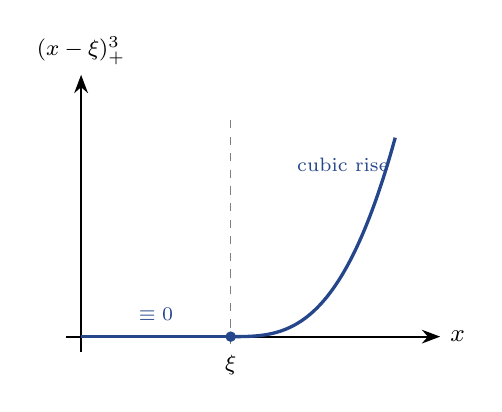
\begin{tikzpicture}[scale=0.95,>=Stealth,font=\small]
      \definecolor{cP}{RGB}{38,70,140}
      \draw[->,thick] (-0.2,0)--(4.8,0) node[right]{$x$};
      \draw[->,thick] (0,-0.2)--(0,3.5) node[above,font=\footnotesize]{$(x-\xi)^3_+$};
      \draw[cP,very thick] (0,0)--(2,0);
      \draw[cP,very thick,domain=2:4.2,smooth,samples=40] plot(\x,{0.25*(\x-2)*(\x-2)*(\x-2)});
      \draw[gray,dashed] (2,-0.1)--(2,3.0);
      \node[below,font=\footnotesize] at (2,-0.12) {$\xi$};
      \fill[cP] (2,0) circle(2pt);
      \node[cP,font=\scriptsize] at (1.0,0.3) {$\equiv 0$};
      \node[cP,font=\scriptsize] at (3.5,2.3) {cubic rise};
    \end{tikzpicture}
    \end{center}
    \end{column}
    \begin{column}{0.45\textwidth}
      \begin{readme}[Reading $(x-\xi)^3_+$]
        The ``$+$'' is the \emph{positive part}: the term is $0$ for
        $x\le\xi$ and equals $(x-\xi)^3$ afterwards. Its value, slope
        and curvature are all $0$ at $\xi$, so switching it on adds a
        bend \emph{only to the right} of the knot without breaking
        $C^2$-smoothness.
      \end{readme}
    \end{column}
  \end{columns}
  \begin{takeaway}Full basis for $K$ knots: $\;1,\,x,\,x^2,\,x^3,\,(x-\xi_1)^3_+,\dots,(x-\xi_K)^3_+\;$ --- that is $K+4$ functions, exactly the $K+4$ degrees of freedom of a cubic spline.\end{takeaway}
\end{frame}

\begin{frame}{Adding constraints turns loose pieces into a spline}
  \begin{center}
    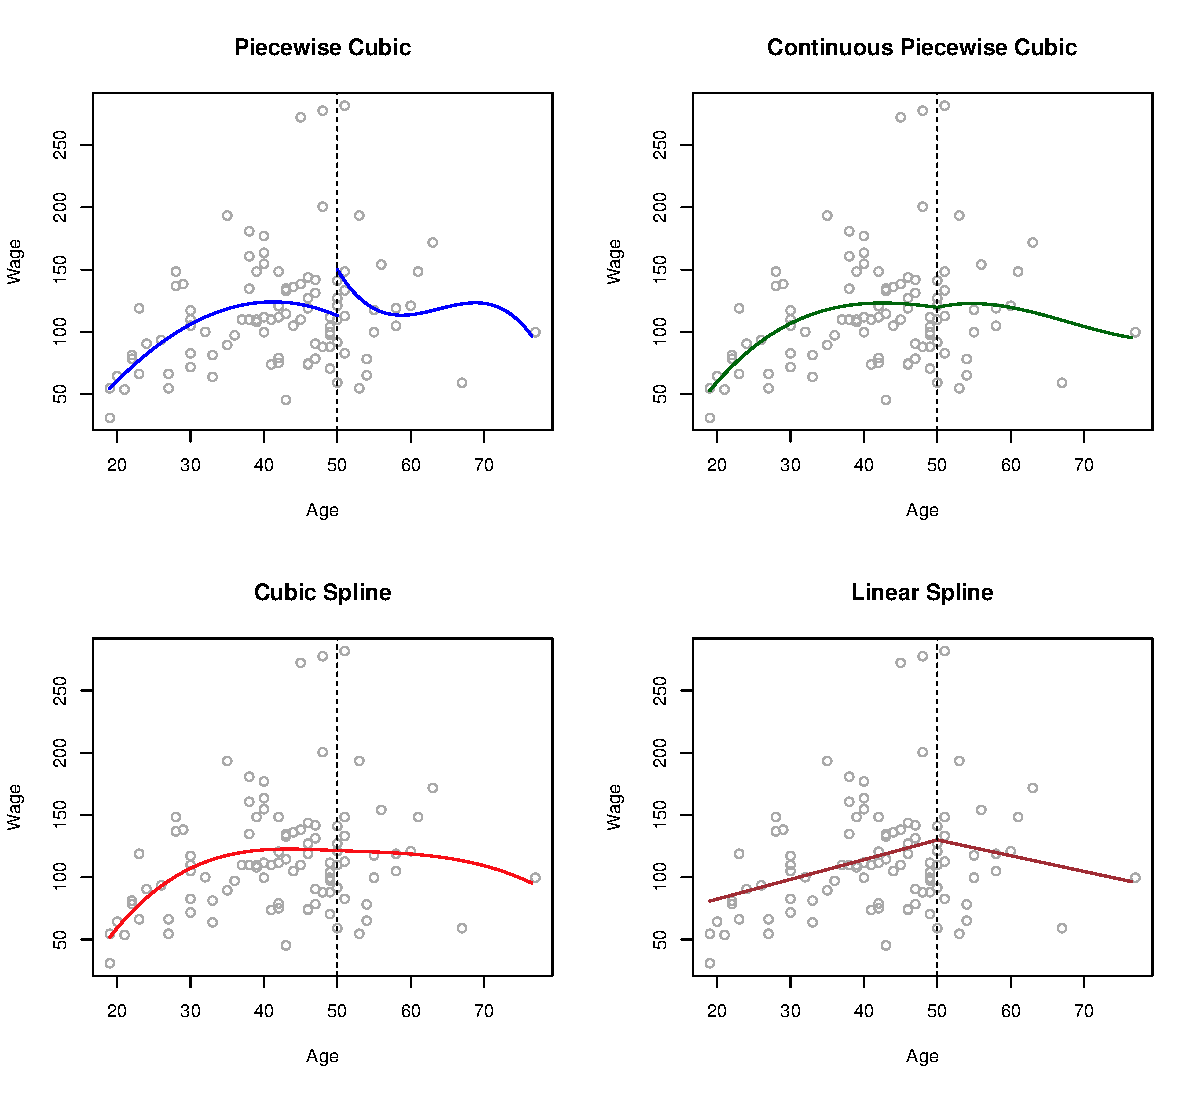
\includegraphics[width=0.92\textwidth,height=0.50\textheight,keepaspectratio]{7_3.pdf}
  \end{center}
  \begin{takeaway}Top-left: unconstrained pieces jump. Adding continuity of value, then slope, then curvature (bottom-left) removes the kinks --- the cubic spline is smoothest.\end{takeaway}
  \islpsource{Figure 7.3}
\end{frame}

% ====================== EXTENDED EXERCISE: Splines ======================
\begin{frame}{Extended Exercise 7.1 --- Regression splines by hand [Math]}
\begin{longexercise}
Build a cubic regression spline for \texttt{wage} on \texttt{age} with $K=3$ interior knots $\xi_1=25<\xi_2=40<\xi_3=60$.
\begin{enumerate}
  \item Write the truncated-power basis and state the total degrees of freedom.
  \item The fitted function is
  \[ \hat g(x)=40+0.5\,x+0.0004\,(x-25)^3_+ -0.0002\,(x-40)^3_+ +0.0003\,(x-60)^3_+ . \]
  Evaluate $\hat g(50)$.
  \item Show that $\hat g,\hat g',\hat g''$ are continuous at $\xi_2=40$ but $\hat g'''$ jumps.
  \item How many degrees of freedom does a \emph{natural} cubic spline with the same three knots use? Explain the difference.
\end{enumerate}
\end{longexercise}
\end{frame}

\begin{frame}{Solution --- Extended Exercise 7.1 (1/3)}
\begin{solutionbox}
\textbf{(a) Truncated-power basis.} With $K=3$ knots the cubic-spline basis is
\[ 1,\ x,\ x^2,\ x^3,\ (x-\xi_1)^3_+,\ (x-\xi_2)^3_+,\ (x-\xi_3)^3_+, \]
so a fitted spline is $\hat g(x)=\beta_0+\beta_1x+\beta_2x^2+\beta_3x^3+\sum_{k=1}^{3}\beta_{3+k}(x-\xi_k)^3_+$.

\medskip
\textbf{Degrees of freedom.} Four base terms plus one per knot: $4+K=7$. Equivalently, a free cubic in each of the $K+1=4$ regions has $4\cdot4=16$ parameters, minus $3$ continuity constraints ($g,g',g''$) at each of the $3$ knots: $16-9=7$.

\medskip
\emph{Why this basis works:} each $(x-\xi_k)^3_+$ has value, slope and curvature $0$ at its knot, so it bends the fit only to the \emph{right} of $\xi_k$ without breaking smoothness --- plain OLS on these $7$ columns automatically yields a $C^2$ piecewise cubic.
\end{solutionbox}
\end{frame}

\begin{frame}{Solution --- Extended Exercise 7.1 (2/3)}
\begin{solutionbox}
\textbf{(b) Evaluate $\hat g(50)$.} Here the quadratic and cubic \emph{base} coefficients happen to be zero, so only the linear base term and the \emph{active} truncated terms contribute. At $x=50$ the knots $25$ and $40$ are exceeded but $60$ is not:
\[ (50-25)^3=25^3=15625,\quad (50-40)^3=10^3=1000,\quad (50-60)^3_+=0. \]
Therefore
\begin{align*}
\hat g(50)&=40+0.5(50)+0.0004(15625)-0.0002(1000)+0.0003(0)\\
&=40+25+6.25-0.20+0 = \mathbf{71.05}.
\end{align*}
Only the basis functions ``switched on'' at $x=50$ enter the sum --- this locality is the point of the truncated basis.

\medskip
\textit{Common mistake:} evaluating the third term as $(50-60)^3=(-10)^3=-1000$ instead of $0$. The ``$+$'' truncation zeroes the term for $x\le 60$; forgetting it would give the wrong value $71.05-0.30=70.75$.
\end{solutionbox}
\end{frame}

\begin{frame}{Solution --- Extended Exercise 7.1 (3/3)}
\begin{solutionbox}
\textbf{(c) Continuity at $\xi_2=40$.} Only the term $t(x)=(x-40)^3_+$ changes behaviour there. With $t'=3(x-40)^2_+$ and $t''=6(x-40)_+$, its one-sided limits at $x=40$ are
\[
\begin{array}{c|ccc}
 & t & t' & t'' \\\hline
x\to40^- & 0 & 0 & 0\\
x\to40^+ & 0 & 0 & 0
\end{array}
\]
so $\hat g,\hat g',\hat g''$ are continuous. But $t'''=6\cdot\mathbf{1}\{x>40\}$ jumps from $0$ to $6$, hence $\hat g'''$ is discontinuous --- the signature of a cubic spline (continuous curvature, kinked third derivative).

\medskip
\textbf{(d) Natural cubic spline.} It is forced \emph{linear} beyond the two boundary knots, imposing $2$ extra constraints at each end ($g''=g'''=0$), i.e.\ $4$ fewer df: $7-4=\mathbf{3}$. A natural spline spends its budget in the interior and is far more stable at the edges.
\end{solutionbox}
\end{frame}

\end{document}
